\documentclass[11pt,letterpaper]{article}
\usepackage[top=1in,bottom=1in,left=1in,right=1in]{geometry}
\usepackage{graphicx}
\usepackage{booktabs}
\usepackage{amsmath}
\usepackage{float}
\usepackage{caption}
\usepackage{subcaption}
\usepackage{microtype}
\usepackage[hidelinks,unicode]{hyperref}
\usepackage{parskip}
\setlength{\parskip}{5pt}
\setlength{\parindent}{0pt}

\captionsetup{font=small, labelfont=bf, skip=4pt}

\begin{document}

% ── Title ──────────────────────────────────────────────────────────────────
\begin{center}
  {\large\bfseries Multivariate Structure and Prediction in the\\[2pt]
   Communities and Crime Dataset}\\[8pt]
  Sidharth Saha \quad Shen-Ching Feng \quad Beckham Wee \quad Joe Wang\\[3pt]
  {\small STAT\,32950 / STAT\,24620 / FINM\,34700 \quad Spring 2026}
\end{center}
\vspace{2pt}\hrule\vspace{8pt}

% ── 1. Introduction ─────────────────────────────────────────────────────────
\section{Introduction}

We investigate what community-level multivariate patterns are associated with above-median violent crime, and how well those patterns can predict the binary outcome \texttt{HighViolentCrime}. The Communities and Crime dataset combines 1990 U.S.\ Census, 1990 LEMAS, and 1995 FBI Uniform Crime Report data for 1{,}994 communities across 100 normalized socioeconomic, demographic, family-structure, housing, and law-enforcement predictors. Because many predictors are highly correlated—capturing overlapping aspects of community disadvantage—multivariate dimension-reduction methods are well-suited to uncover latent structure before prediction.

We apply five families of analysis: principal component analysis (PCA), factor analysis (FA), $K$-means clustering, logistic regression and LDA, and regularized logistic regression. Together these methods allow us to characterize community structure, connect that structure to the crime outcome, and assess predictive performance across different input representations.

% ── 2. Data and Preprocessing ───────────────────────────────────────────────
\section{Data and Preprocessing}

The dataset contains 1{,}994 communities and 102 columns: 100 predictors, the continuous outcome \texttt{ViolentCrimesPerPop} (normalized per-capita violent crime), and the binary label \texttt{HighViolentCrime} (High if above the sample median). The class split is approximately balanced: 993 High and 1{,}001 Low communities. Predictors span six thematic groups—population and urbanization, demographic composition, income and poverty, education and employment, family structure, and housing and residential stability—all pre-normalized to $[0,1]$ in the provided dataset.

Variables with more than 20\% missingness were removed prior to delivery; remaining numeric missing values were median-imputed. All predictors were standardized to zero mean and unit variance before PCA and factor analysis, because the variables represent different measurement types and retain unequal variance after normalization. The same standardized matrix is used as input for all models. The 70/30 stratified train-test split (1{,}395 train / 599 test) is held fixed across all classifiers using \texttt{random\_state\,=\,42}.

Figure~\ref{fig:eda} illustrates the distribution of six key predictors broken out by crime class. High violent-crime communities tend to have lower median income, fewer children in two-parent families, higher poverty rates, lower bachelor's-degree attainment, lower owner-occupied housing, and higher divorce rates—previewing the dimensions that dominate the multivariate analyses below.

\begin{figure}[htbp]
  \centering
  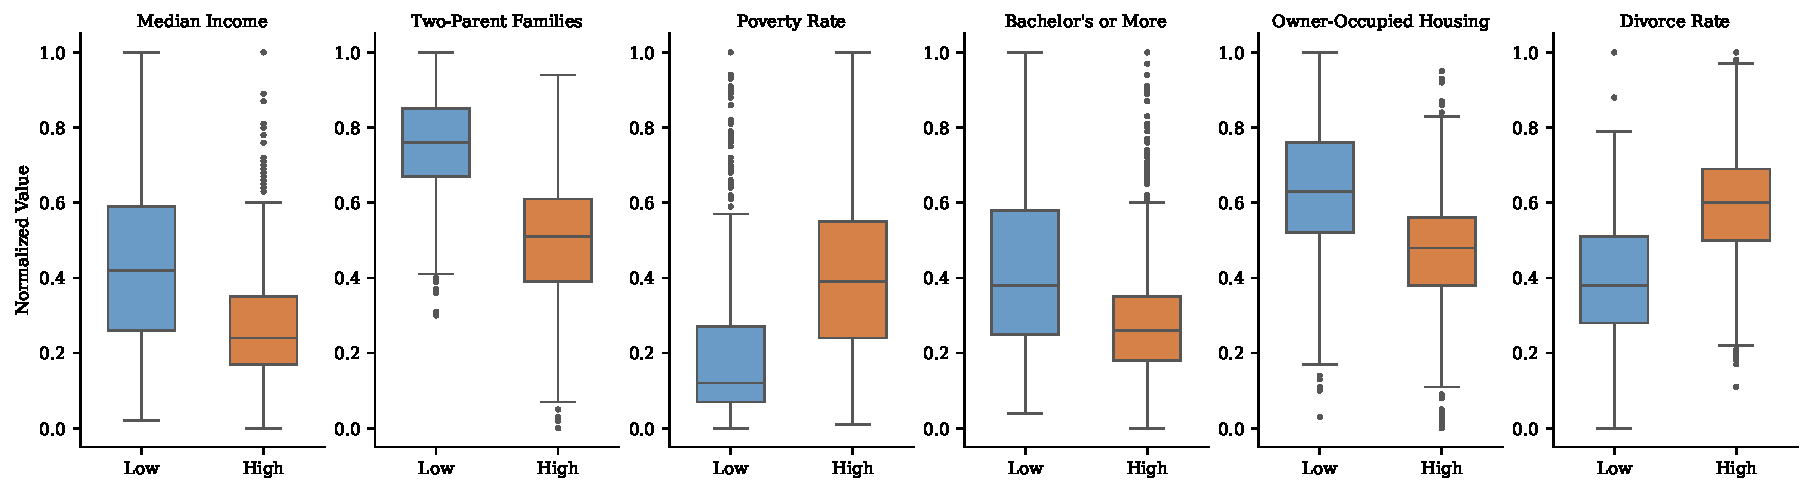
\includegraphics[width=\linewidth]{figures/fig_eda.pdf}
  \caption{Selected predictors by violent-crime class. Each panel shows the distribution
           of a normalized predictor for Low (blue) and High (orange) crime communities.}
  \label{fig:eda}
\end{figure}

% ── 3. Methods and Results ──────────────────────────────────────────────────
\section{Methods and Results}

\subsection{Principal Component Analysis}

Correlation PCA was fit on all 100 standardized predictors. Figure~\ref{fig:pca}(a) shows the scree plot: PC1 alone explains 28.0\% of total variance, and the first 11 components together explain 80\%. The scree elbow and the 80\% threshold both support retaining 11--13 components for downstream use. PC2 explains 8.8\%.

PC1 is labeled \emph{economic advantage and family stability}: it has large positive loadings on median income, per-capita income, bachelor's-degree attainment, and the share of children in two-parent families, and large negative loadings on poverty rate, public assistance receipt, and divorce rate. PC2 captures \emph{immigration and language composition}. Figure~\ref{fig:pca}(b) shows the PC1--PC2 score plot colored by \texttt{HighViolentCrime}. High-crime communities concentrate at negative PC1 values, confirming that economic disadvantage and family instability are the dominant discriminating dimensions.

\begin{figure}[htbp]
  \centering
  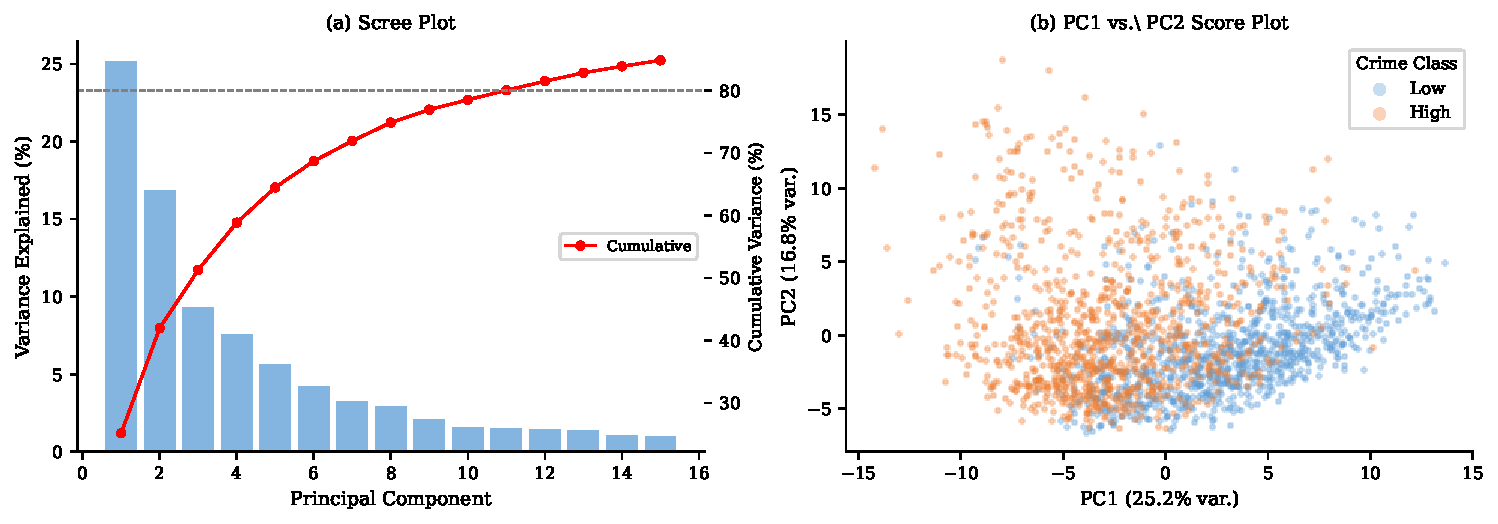
\includegraphics[width=\linewidth]{figures/fig_pca.pdf}
  \caption{PCA results. \textbf{(a)}~Scree plot: individual (bars) and cumulative (line)
           variance explained by the first 15 PCs; dashed line marks 80\%.
           \textbf{(b)}~PC1 vs.\ PC2 score plot colored by violent-crime class.}
  \label{fig:pca}
\end{figure}

\subsection{Factor Analysis}

A 7-factor varimax solution was selected based on parallel analysis and RMSR diagnostics applied to the same standardized predictor matrix. The seven factors have clear thematic interpretations: (1)~immigration and language composition, (2)~income and housing value, (3)~urban size and concentrated disadvantage, (4)~household size, (5)~youth and young-adult composition, (6)~family structure and community composition, and (7)~older residential stability.

Factor~6 (family structure) shows the strongest association with \texttt{HighViolentCrime}: communities with above-median crime score 1.075 points higher on Factor~6 than below-median communities. Factors~2 and~3 also show notable mean differences (0.531 and 0.369, respectively). These factor labels are working interpretations of loading patterns, not causal claims.

\subsection{K-Means Clustering}

K-means was fit on the first 11 PCA scores (those explaining 80\% of variance) with $K$ selected by the highest average silhouette score across $K = 2$--$20$; $K=3$ was optimal. Figure~\ref{fig:clusters} shows the three clusters in PC1--PC2 space. The lowest-crime cluster (Cluster~1) has positive mean PC1 scores and the highest share of economic advantage. The highest-crime cluster has strongly negative PC1 scores and elevated PC2 scores, indicating lower economic advantage and a distinct immigration and language composition. The intermediate cluster falls between these extremes. The three clusters thus form a clean low-to-high crime gradient along PC1, directly connecting the unsupervised structure to the outcome.

\begin{figure}[htbp]
  \centering
  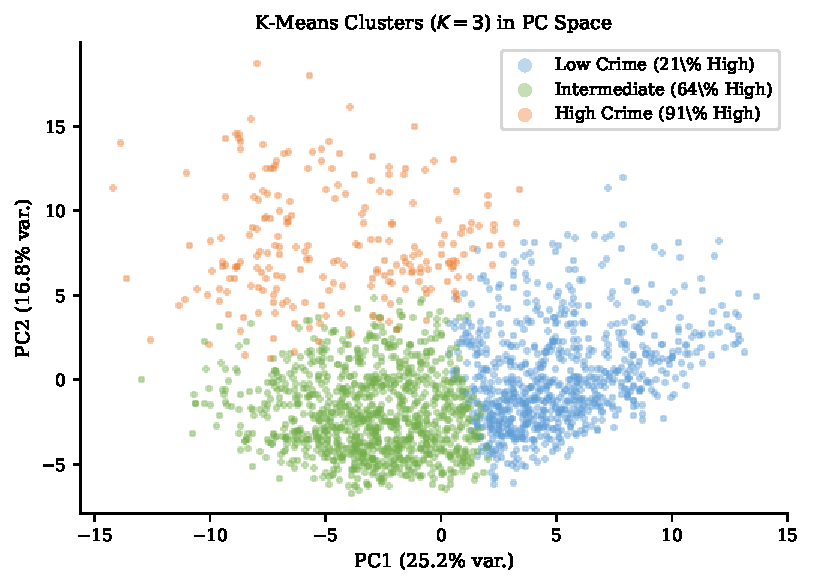
\includegraphics[width=0.62\linewidth]{figures/fig_clusters.pdf}
  \caption{K-means clusters ($K=3$) in PC1--PC2 space.
           Percentage in parentheses gives the share of High violent-crime communities
           within each cluster.}
  \label{fig:clusters}
\end{figure}

\subsection{Classification}

Five classifiers were evaluated using the fixed 70/30 split. Three logistic regression models used different input representations: the original 100 standardized predictors, the 11 retained PCA scores, and the 7 factor scores. Two LDA models used the PCA and factor scores (lower-dimensional inputs reduce collinearity for LDA's covariance estimation).

Table~\ref{tab:classification} reports performance on the held-out test set. ROC-AUC ranges from 0.905 to 0.913 across the five unpenalized models. The logistic model on original predictors achieves accuracy 0.846; the factor-score logistic model achieves the highest AUC (0.913) with only 7 inputs. Notably, dimension reduction to 11 PCA scores or 7 factor scores does not degrade predictive accuracy relative to the full 100-predictor model, indicating that the predictive signal is well-captured by the leading components. LDA performs marginally below logistic regression, which is consistent with LDA's equal-covariance assumption being only approximately satisfied.

\subsection{Regularization}

Ridge, lasso, and elastic-net logistic regression were fit on the full 100-predictor matrix with regularization strength selected by 5-fold cross-validated ROC-AUC. Ridge achieves the best overall AUC (0.915). Lasso attains AUC~0.913 while retaining only 47 of 100 predictors, and elastic net retains 44. The selected lasso predictors include investment income, family-structure variables, housing vacancy, residential mobility, and law-enforcement indicators. The gains over unpenalized logistic regression are modest, suggesting the predictive signal is strong enough that regularization improves stability more than accuracy. Rows for Ridge, Lasso, and Elastic Net appear in Table~\ref{tab:classification} alongside the unpenalized models.

\begin{table}[htbp]
  \centering
  \small
  \caption{Classification performance on held-out test set ($n=599$). Parentheses after
           regularized model names give the number of nonzero coefficients.
           Best AUC in each group is \textbf{bold}.}
  \label{tab:classification}
  \begin{tabular}{lcccc}
    \toprule
    Model & Accuracy & Sensitivity & Specificity & AUC \\
    \midrule
    Logistic (Original)  & 0.846 & 0.822 & 0.870 & 0.912 \\
    Logistic (PCA)       & 0.830 & 0.826 & 0.834 & 0.912 \\
    Logistic (Factors)   & 0.835 & 0.832 & 0.837 & \textbf{0.913} \\
    LDA (PCA)            & 0.825 & 0.799 & 0.850 & 0.905 \\
    LDA (Factors)        & 0.825 & 0.805 & 0.844 & 0.906 \\
    \midrule
    Ridge (100 coef.)    & 0.841 & 0.822 & 0.860 & \textbf{0.915} \\
    Lasso (47 coef.)     & 0.848 & 0.822 & 0.874 & 0.913 \\
    Elastic Net (44 coef.)& 0.838 & 0.819 & 0.857 & 0.914 \\
    \bottomrule
  \end{tabular}
\end{table}

\begin{figure}[htbp]
  \centering
  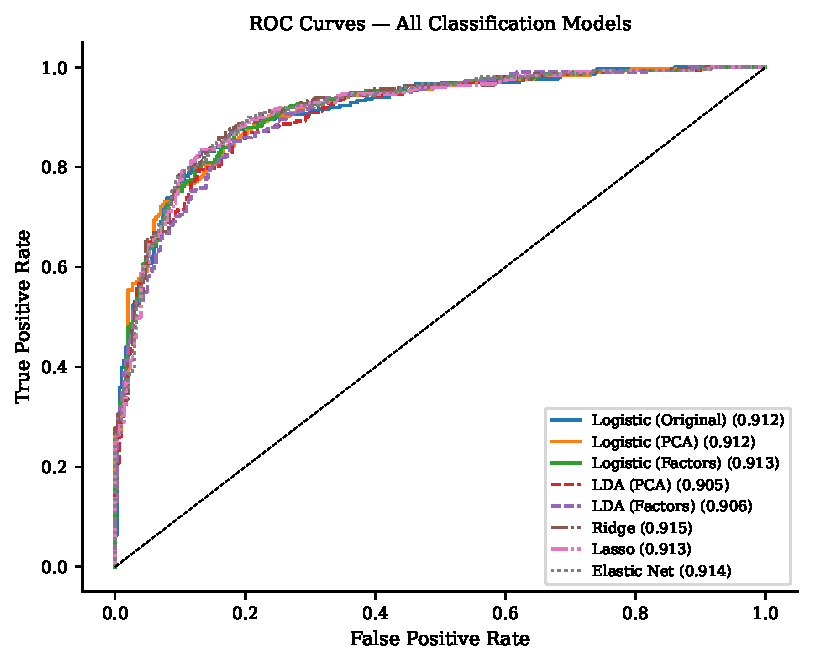
\includegraphics[width=0.72\linewidth]{figures/fig_roc.pdf}
  \caption{ROC curves for all eight models on the held-out test set.
           AUC values are shown in the legend.}
  \label{fig:roc}
\end{figure}

% ── 4. Comparison Across Methods ────────────────────────────────────────────
\section{Comparison Across Methods}

Every method identifies the same structural account of the data. PCA and factor analysis independently recover the same primary axis: economic disadvantage and family instability (PC1; Factor~6 and Factor~2). This is not a property of a single algorithmic choice; it emerges from two distinct decompositions of the correlation matrix, providing strong evidence that this axis reflects genuine variation in the data rather than a modeling artifact.

K-means confirms the structure by producing three clusters that follow a monotone crime gradient along PC1. The cluster memberships are predictable from the same variables that dominate PC1 and Factor~6, meaning the unsupervised partition is directly aligned with the supervised outcome.

Prediction performance is consistent across all input representations: 11 PCA scores, 7 factor scores, and 100 original predictors all yield ROC-AUC in the 0.905--0.915 range. This suggests that the predictive content of the full predictor set is almost entirely contained in the few leading dimensions of variation—the same dimensions identified by PCA and factor analysis as substantively meaningful. Regularization offers marginal additional gains; the main benefit of lasso is parsimonious variable selection, not improved discrimination.

% ── 5. Limitations ──────────────────────────────────────────────────────────
\section{Limitations}

All results are observational and ecological: associations between community-level variables and crime rates do not imply individual-level causal effects. Crime statistics reflect reported and recorded offenses, which are sensitive to policing practices and community trust. The predictor variables come from 1990 while the crime outcome comes from 1995; five-year confounders are not captured. Demographic variables including racial composition appear as predictive signals in lasso coefficients and cluster profiles; these reflect systemic socioeconomic patterns and must not be interpreted as group-level propensities. Finally, results are specific to early-1990s U.S.\ communities and may not generalize to other settings or time periods.


\end{document}
